\documentclass[10pt]{beamer}
\usetheme{Malmoe}
\usepackage[T2A]{fontenc}
\usepackage[utf8]{inputenc}
\usepackage[russian, english]{babel} % Языки документа
\usepackage{amsmath,pgfplots,booktabs,hyperref,graphicx}
\usepackage[style=verbose-ibid,backend=biber]{biblatex}
\addbibresource{references.bib}

% График воды (рендерится через Python → murray_flow_ratio.pdf)
\usepackage{graphicx}

% Настройка заголовков
\setbeamerfont{title}{size=\LARGE}
\setbeamerfont{frametitle}{size=\large}

% Титульный
\title{Инструменты разделения редких\\ и неравномерно распределённых ресурсов}
\subtitle{25-минутный доклад для экономистов-математиков}
\author{Ваше имя}
\date{\today}

\begin{document}

\maketitle

% ================= СЛАЙД 2 — КРЮЧОК =================
\begin{frame}{Почему это не про «рынок или государство»}
  \begin{columns}
    \column{0.6\textwidth}
    \textbf{Крючок:}
    \begin{itemize}
      \item Население хочет \textbf{тепло}, а не нефть
      \item Спрос на нефть — \textbf{производный}: $D_{oil}(p) = \sum_i \alpha_i D_i(p_i)$
      \item Конкуренция — на уровне \textbf{фирм и государств}, не домохозяйств
    \end{itemize}

    \column{0.35\textwidth}
    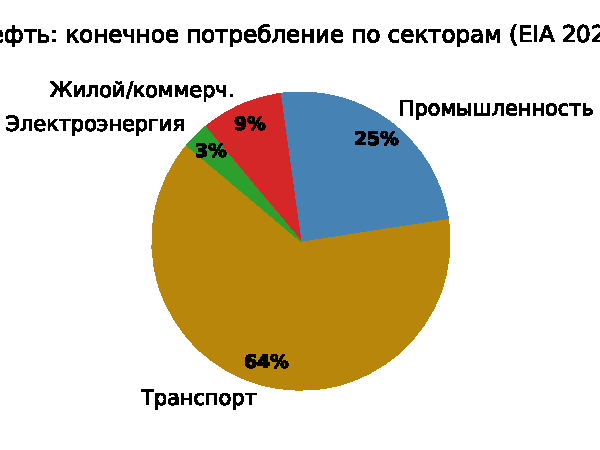
\includegraphics[width=\linewidth]{oil_sector_pie.pdf}
  \end{columns}
  \vspace{0.5cm}
  \begin{alertblock}{}
    «Одна и та же идея — рынок прав — даёт противоположные результаты» (Чили vs Австралия)
  \end{alertblock}
\end{frame}

% ================= СЛАЙД 3 — ТРИ ОСИ =================
\begin{frame}{Три оси — не путать}
  \begin{tabular}{@{}llp{5cm}@{}}
    \toprule
    \textbf{Ось} & \textbf{Формально} & \textbf{Измеримый индикатор} \\
    \midrule
    Ограниченность (flow) & $\dot{Q} \le R$ & $R/Q$ (горизонт исчерпания) \\
    Редкость (scarcity)   & $D(0) > Q$ & $S = D(0)-Q$, эластичность предложения \\
    Неравномерность       & Концентрация прав & HHI по лицензиям, индекс Джини \\
    \bottomrule
  \end{tabular}

  \vspace{0.6cm}
  \begin{exampleblock}{}
    Воздух в чистой местности: $S(0) \le 0$ — \textbf{не редок}, инструменты распределения не нужны.
  \end{exampleblock}
\end{frame}

% ================= СЛАЙД 4 — МАТРИЦА =================
\begin{frame}{Матрица исключаемость / соперничество}
  \centering
  \begin{tikzpicture}
    \draw[->] (0,0) -- (6,0) node[right] {Исключаемость};
    \draw[->] (0,0) -- (0,5) node[above] {Соперничество};
    \draw[thick] (0,0) rectangle (3,3) node[midway] {Частные};
    \draw[thick] (3,0) rectangle (6,3) node[midway] {Клубные};
    \draw[thick] (0,3) rectangle (3,6) node[midway] {Общие (commons)};
    \draw[thick] (3,3) rectangle (6,6) node[midway] {Открытый доступ};
    \node at (1.5,1.5) {рынок};
    \node at (4.5,1.5) {рынок / гос.};
    \node at (1.5,4.5) {общинные правила};
    \node at (4.5,4.5) {деградация};
  \end{tikzpicture}
\end{frame}

% ================= СЛАЙД 5 — ИНСТРУМЕНТАРИЙ =================
\begin{frame}{Инструментарий — три блока}
  \begin{columns}
    \column{0.3\textwidth}
    \textbf{Собственность}
    \begin{itemize}
      \item Частная (ITQ)
      \item Государственная (концессии)
      \item Commons (Остром)
    \end{itemize}

    \column{0.3\textwidth}
    \textbf{Распределение}
    \begin{itemize}
      \item Аукцион (Vickrey)
      \item Очередь / лотерея
      \item Переуступаемые квоты
    \end{itemize}

    \column{0.3\textwidth}
    \textbf{Ограничение}
    \begin{itemize}
      \item Налог Пигу
      \item Cap-and-trade
      \item Технология / лимит
    \end{itemize}
  \end{columns}
\end{frame}

% ================= СЛАЙД 6 — ВОДА (ЧИЛИ/АВСТРАЛИЯ) =================
\begin{frame}{Вода: Чили (1981) vs Австралия (Murray--Darling)}
  \begin{columns}
    \column{0.48\textwidth}
    \begin{tabular}{@{}ll@{}}
      \toprule
      \textbf{Чили} & \textbf{Австралия} \\
      \midrule
      Частная, отделена от земли & Государственная (entitlement) \\
      Аукцион + рынок & Бесплатная аллокация + trade \\
      \textbf{Нет потолка} & \textbf{Cap} (экология) \\
      Падение стока (Petorca) & Смягчение засухи \\
      \bottomrule
    \end{tabular}
    \footnotesize \textit{Источники: Bauer (2004), Budds (2008), Grafton et al. (2012), MDBA (2020)}

    \column{0.48\textwidth}
    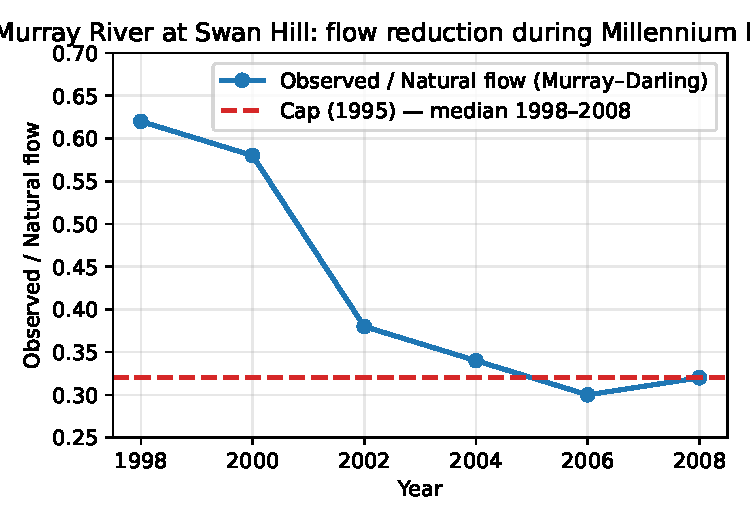
\includegraphics[width=\linewidth]{murray_flow_ratio.pdf}
  \end{columns}
\end{frame}

% ================= СЛАЙД 7 — ФОРМАЛЬНАЯ СУТЬ =================
\begin{frame}{Формальная суть}
  \begin{columns}
    \column{0.5\textwidth}
    \textbf{Чили — без потолка}
    $$q_i \ge 0,\quad \sum q_i \text{ не ограничен}$$
    Цена $\to$ предельные издержки, \textbf{не} ценность воды.

    \column{0.5\textwidth}
    \textbf{Австралия — внутри Cap}
    $$\bar{Q} = \sum q_i,\quad q_i = e_i \cdot \frac{\bar{Q}}{\sum e_i}$$
    Торговля \textit{долей} потолка. В засуху $\bar{Q}$ падает — цена растёт, \textbf{но объём $\le \bar{Q}$}.
  \end{columns}
  \vspace{0.5cm}
  \begin{alertblock}{}
    Одна и та же конструкция (торгуемые права) $\Rightarrow$ противоположные результаты.
  \end{alertblock}
\end{frame}

% ================= СЛАЙД 8 — ИНСТРУМЕНТАРИЙ (ТАБЛИЦА) =================
\begin{frame}{Что это значит для выбора инструмента}
  \centering
  \begin{tabular}{@{}ccc@{}}
    \toprule
    Режим & Инструмент & Условие работы \\
    \midrule
    Частная & Рынок & Спецификация прав \\
    Государственная & Cap + trade & Измеримый потолок \\
    Commons & Правила сообщества & Границы + мониторинг \\
    \bottomrule
  \end{tabular}
  \vspace{0.8cm}
  \begin{block}{}
    \textbf{Инструмент не выбирается — он следует из того, какой параметр вы можете измерить и удержать.}
  \end{block}
\end{frame}

% ================= СЛАЙД 9 — ВАЙЦМАН =================
\begin{frame}{Правило Вайцмана (1974): цена vs количество}
  \begin{columns}
    \column{0.5\textwidth}
    \begin{tikzpicture}[scale=0.7]
      \begin{axis}[axis lines=left, width=0.9\linewidth]
        \addplot[blue, thick] coordinates {(0,8) (6,2)} node[midway,above] {$MB$};
        \addplot[red, thick]  coordinates {(0,2) (6,8)} node[midway,above] {$MC$};
        \addplot[dashed] coordinates {(4,0) (4,6)};
        \node at (2.5,5) {налог};
      \end{axis}
    \end{tikzpicture}
    \column{0.5\textwidth}
    \begin{tikzpicture}[scale=0.7]
      \begin{axis}[axis lines=left, width=0.9\linewidth]
        \addplot[blue, thick] coordinates {(0,8) (6,5)} node[midway,above] {$MB$};
        \addplot[red, thick]  coordinates {(0,4) (6,7)} node[midway,above] {$MC$};
        \addplot[dashed] coordinates {(4,0) (4,6)};
        \node at (2.5,5.5) {квота};
      \end{axis}
    \end{tikzpicture}
  \end{columns}
  \vspace{0.5cm}
  \begin{block}{}
    $e < f$ (MB пологая) $\Rightarrow$ \textbf{налог}; $e > f$ (MB крутая) $\Rightarrow$ \textbf{квота}. \\
    При «толстых хвостах» — квота (Weitzman 2009).
  \end{block}
  \footnotesize $\displaystyle \frac{L_{\text{price}}}{L_{\text{quota}}} = \left( \frac{e}{f} \right)^2$ (квадратичные потери, сдвиг MC)
\end{frame}

% ================= СЛАЙД 10 — UNOS =================
\begin{frame}{UNOS: распределение органов — MELD 3.0 (2023)}
  \begin{columns}
    \column{0.6\textwidth}
    \textbf{Компоненты MELD 3.0:}
    \begin{itemize}
      \item Билирубин (лог), МНО (лог), Креатинин (лог) + диализ
      \item Пол: женщина $+1.33$
      \item Исключения: HCC
    \end{itemize}
    \textbf{Непрерывное распределение (2021--2023):}
    \begin{itemize}
      \item Убраны границы DSA
      \item Расстояние от донора — компонент балла
      \item Баланс: срочность vs выживаемость
    \end{itemize}
    %\column{0.35\textwidth}
    %\includegraphics[width=\linewidth]{optn_logo.pdf}
  \end{columns}
  \vspace{0.5cm}
  \begin{alertblock}{}
    Третий полюс: \textbf{приоритизация без денег} (не рынок, не государство).
  \end{alertblock}
\end{frame}

% ================= СЛАЙД 11 — ЗАКРЫТИЕ =================
\begin{frame}{Синтез}
  \centering
  \begin{tabular}{@{}ccc@{}}
    \toprule
    Ресурс & Инструмент & Почему \\
    \midrule
    Вода (Чили) & Рынок & Нет потолка — цена не останавливает \\
    Вода (Австралия) & Cap + trade & Потолок — цена останавливает \\
    Углерод & Вайцман & Крутая MB — квота \\
    Органы & UNOS (MELD) & Нет рынка — приоритет \\
    \bottomrule
  \end{tabular}

  \vspace{0.8cm}
  \begin{block}{}
    \textbf{Набор инструментов:} собственность $\to$ распределение $\to$ ограничение $\to$ аукцион $\to$ паросочетание. \\
    Выбор определяет \textbf{не ресурс}, а геометрия кривых и измеримость параметров.
  \end{block}
\end{frame}

% ================= СЛАЙД 12 — ВОПРОС + ИСТОЧНИКИ =================
\begin{frame}{Вопрос залу \& источники}
  \begin{columns}
    \column{0.6\textwidth}
    \textbf{Вопрос:} \\
    На каком ресурсе из перечисленных вы бы \textbf{запретили} цену? \\
    (вода, органы, радиочастоты, углерод, земля)
    
    \vspace{0.5cm}
    \textbf{Основные источники:}
    \begin{itemize}
      \item Bauer (2004) — \textit{Against the Current}
      \item Budds (2008) — \textit{Geoforum}
      \item Grafton et al. (2012) — \textit{Water Planning and Hydro-Climatic Change}
      \item Weitzman (1974) — \textit{RES}
      \item UNOS/OPTN (2023) — Policy 4.0
    \end{itemize}

    %\column{0.35\textwidth}
    %\includegraphics[width=\linewidth]{water_capital.pdf}
  \end{columns}
\end{frame}

\end{document}
